% This file was created with tikzplotlib v0.10.1.
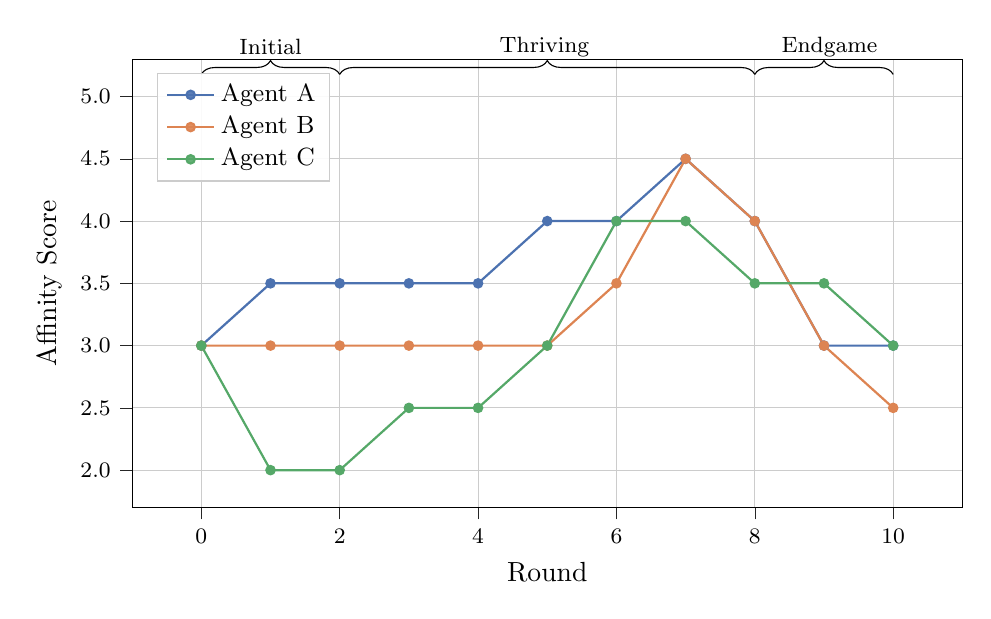
\begin{tikzpicture}

\definecolor{darkslategrey38}{RGB}{38,38,38}
\definecolor{lightgrey204}{RGB}{204,204,204}
\definecolor{mediumseagreen85168104}{RGB}{85,168,104}
\definecolor{peru22113282}{RGB}{221,132,82}
\definecolor{steelblue76114176}{RGB}{76,114,176}

% \begin{axis}[
% axis line style={lightgrey204},
% legend cell align={left},
% legend style={fill opacity=0.8, draw opacity=1, text opacity=1, draw=lightgrey204},
% tick align=outside,
% title={Average Affinity Rating},
% x grid style={lightgrey204},
% xmajorgrids,
% xmajorticks=false,
% xmin=-0.5, xmax=10.5,
% xtick style={color=darkslategrey38},
% y grid style={lightgrey204},
% ylabel=\textcolor{darkslategrey38}{Mean Rating},
% ymajorgrids,
% ymajorticks=false,
% ymin=1.875, ymax=4.625,
% ytick style={color=darkslategrey38}
% ]
\begin{axis}[
legend cell align={left},
legend style={
  fill opacity=0.8,
  draw opacity=1,
  text opacity=1,
  at={(0.03,0.97)},
  anchor=north west,
  draw=lightgrey204,
  font=\small
},
width=1.\textwidth,    % 设置宽度
    height=0.6\textwidth,  % 16:9比例
    axis line style={black},
    legend style={fill opacity=0.9, draw opacity=1, text opacity=1, draw=lightgrey204},
    tick align=outside,     % 刻度线向外
    xtick={0,2,4,6,8,10},
    % xticklabels={Initial,Flourishing,Endgame},
    xticklabel style={font=\footnotesize},
    y grid style={lightgrey204},
    xlabel=Round,
    xlabel style={font=\footnotesize},
    ylabel=Affinity Score,
   ylabel style={font=\footnotesize,
            inner sep=0pt,    % 减少标签和轴的距离
            yshift=-5pt       % 微调标签位置
        },
    ymajorgrids,
    ytick={2.0,2.5,3.0,3.5,4.0,4.5,5.0},
    yticklabel style={font=\footnotesize,
    /pgf/number format/.cd,
    fixed,
    precision=1,
    zerofill},
    ymin=2, ymax=5,
    xtick style={color=darkslategrey38},
    ytick style={color=darkslategrey38},
    enlarge x limits=0.1,
    enlarge y limits=0.1,
    grid=major,
    grid style={lightgrey204},
    tick style={color=darkslategrey38},
    axis lines=box,        % 保持完整边框
    x axis line style={black},
    y axis line style={black},
    % 控制刻度线的显示
    tick pos=left,         % y轴刻度线只在左侧显示
    xtick pos=bottom,      % x轴刻度线只在底部显示
    clip=false              % 裁剪超出的内容
]
\addplot [thick, steelblue76114176, mark=*, mark size=1.5, mark options={solid}]
table {%
0 3
1 3.5
2 3.5
3 3.5
4 3.5
5 4
6 4
7 4.5
8 4
9 3
10 3
};
\addlegendentry{Agent A}
\addplot [thick, peru22113282, mark=*, mark size=1.5, mark options={solid}]
table {%
0 3
1 3
2 3
3 3
4 3
5 3
6 3.5
7 4.5
8 4
9 3
10 2.5
};
\addlegendentry{Agent B}
\addplot [thick, mediumseagreen85168104, mark=*, mark size=1.5, mark options={solid}]
table {%
0 3
1 2
2 2
3 2.5
4 2.5
5 3
6 4
7 4
8 3.5
9 3.5
10 3
};
\addlegendentry{Agent C}

\draw [decorate, decoration={brace, amplitude=5pt},yshift=8pt] (axis cs:0,5) -- (axis cs:2,5) node [black,midway,yshift=10pt, font=\tiny] {\footnotesize Initial};
\draw [decorate, decoration={brace, amplitude=5pt},yshift=8pt] (axis cs:2,5) -- (axis cs:8,5) node [black,midway,yshift=10pt, font=\tiny,xshift=-1pt] {\footnotesize Thriving};
\draw [decorate, decoration={brace, amplitude=5pt},yshift=8pt] (axis cs:8,5) -- (axis cs:10,5) node [black,midway,yshift=10pt, font=\tiny,xshift=2pt] {\footnotesize Endgame};

\end{axis}

\end{tikzpicture}
